\PassOptionsToPackage{unicode=true}{hyperref} % options for packages loaded elsewhere
\PassOptionsToPackage{hyphens}{url}
%
\documentclass[ignorenonframetext,]{beamer}
\usepackage{pgfpages}
\setbeamertemplate{caption}[numbered]
\setbeamertemplate{caption label separator}{: }
\setbeamercolor{caption name}{fg=normal text.fg}
\beamertemplatenavigationsymbolsempty
% Prevent slide breaks in the middle of a paragraph:
\widowpenalties 1 10000
\raggedbottom
\setbeamertemplate{part page}{
\centering
\begin{beamercolorbox}[sep=16pt,center]{part title}
  \usebeamerfont{part title}\insertpart\par
\end{beamercolorbox}
}
\setbeamertemplate{section page}{
\centering
\begin{beamercolorbox}[sep=12pt,center]{part title}
  \usebeamerfont{section title}\insertsection\par
\end{beamercolorbox}
}
\setbeamertemplate{subsection page}{
\centering
\begin{beamercolorbox}[sep=8pt,center]{part title}
  \usebeamerfont{subsection title}\insertsubsection\par
\end{beamercolorbox}
}
\AtBeginPart{
  \frame{\partpage}
}
\AtBeginSection{
  \ifbibliography
  \else
    \frame{\sectionpage}
  \fi
}
\AtBeginSubsection{
  \frame{\subsectionpage}
}
\usepackage{lmodern}
\usepackage{amssymb,amsmath}
\usepackage{ifxetex,ifluatex}
\usepackage{fixltx2e} % provides \textsubscript
\ifnum 0\ifxetex 1\fi\ifluatex 1\fi=0 % if pdftex
  \usepackage[T1]{fontenc}
  \usepackage[utf8]{inputenc}
  \usepackage{textcomp} % provides euro and other symbols
\else % if luatex or xelatex
  \usepackage{unicode-math}
  \defaultfontfeatures{Ligatures=TeX,Scale=MatchLowercase}
\fi
\usetheme[]{boxes}
\usecolortheme{structure}
% use upquote if available, for straight quotes in verbatim environments
\IfFileExists{upquote.sty}{\usepackage{upquote}}{}
% use microtype if available
\IfFileExists{microtype.sty}{%
\usepackage[]{microtype}
\UseMicrotypeSet[protrusion]{basicmath} % disable protrusion for tt fonts
}{}
\IfFileExists{parskip.sty}{%
\usepackage{parskip}
}{% else
\setlength{\parindent}{0pt}
\setlength{\parskip}{6pt plus 2pt minus 1pt}
}
\usepackage{hyperref}
\hypersetup{
            pdftitle={miniBeamer package presentation},
            pdfauthor={Bartek Granat},
            pdfborder={0 0 0},
            breaklinks=true}
\urlstyle{same}  % don't use monospace font for urls
\newif\ifbibliography
\usepackage{color}
\usepackage{fancyvrb}
\newcommand{\VerbBar}{|}
\newcommand{\VERB}{\Verb[commandchars=\\\{\}]}
\DefineVerbatimEnvironment{Highlighting}{Verbatim}{commandchars=\\\{\}}
% Add ',fontsize=\small' for more characters per line
\newenvironment{Shaded}{}{}
\newcommand{\AlertTok}[1]{\textcolor[rgb]{1.00,0.00,0.00}{#1}}
\newcommand{\AnnotationTok}[1]{\textcolor[rgb]{0.00,0.50,0.00}{#1}}
\newcommand{\AttributeTok}[1]{#1}
\newcommand{\BaseNTok}[1]{#1}
\newcommand{\BuiltInTok}[1]{#1}
\newcommand{\CharTok}[1]{\textcolor[rgb]{0.00,0.50,0.50}{#1}}
\newcommand{\CommentTok}[1]{\textcolor[rgb]{0.00,0.50,0.00}{#1}}
\newcommand{\CommentVarTok}[1]{\textcolor[rgb]{0.00,0.50,0.00}{#1}}
\newcommand{\ConstantTok}[1]{#1}
\newcommand{\ControlFlowTok}[1]{\textcolor[rgb]{0.00,0.00,1.00}{#1}}
\newcommand{\DataTypeTok}[1]{#1}
\newcommand{\DecValTok}[1]{#1}
\newcommand{\DocumentationTok}[1]{\textcolor[rgb]{0.00,0.50,0.00}{#1}}
\newcommand{\ErrorTok}[1]{\textcolor[rgb]{1.00,0.00,0.00}{\textbf{#1}}}
\newcommand{\ExtensionTok}[1]{#1}
\newcommand{\FloatTok}[1]{#1}
\newcommand{\FunctionTok}[1]{#1}
\newcommand{\ImportTok}[1]{#1}
\newcommand{\InformationTok}[1]{\textcolor[rgb]{0.00,0.50,0.00}{#1}}
\newcommand{\KeywordTok}[1]{\textcolor[rgb]{0.00,0.00,1.00}{#1}}
\newcommand{\NormalTok}[1]{#1}
\newcommand{\OperatorTok}[1]{#1}
\newcommand{\OtherTok}[1]{\textcolor[rgb]{1.00,0.25,0.00}{#1}}
\newcommand{\PreprocessorTok}[1]{\textcolor[rgb]{1.00,0.25,0.00}{#1}}
\newcommand{\RegionMarkerTok}[1]{#1}
\newcommand{\SpecialCharTok}[1]{\textcolor[rgb]{0.00,0.50,0.50}{#1}}
\newcommand{\SpecialStringTok}[1]{\textcolor[rgb]{0.00,0.50,0.50}{#1}}
\newcommand{\StringTok}[1]{\textcolor[rgb]{0.00,0.50,0.50}{#1}}
\newcommand{\VariableTok}[1]{#1}
\newcommand{\VerbatimStringTok}[1]{\textcolor[rgb]{0.00,0.50,0.50}{#1}}
\newcommand{\WarningTok}[1]{\textcolor[rgb]{0.00,0.50,0.00}{\textbf{#1}}}
\usepackage{longtable,booktabs}
\usepackage{caption}
% These lines are needed to make table captions work with longtable:
\makeatletter
\def\fnum@table{\tablename~\thetable}
\makeatother
\usepackage{graphicx,grffile}
\makeatletter
\def\maxwidth{\ifdim\Gin@nat@width>\linewidth\linewidth\else\Gin@nat@width\fi}
\def\maxheight{\ifdim\Gin@nat@height>\textheight\textheight\else\Gin@nat@height\fi}
\makeatother
% Scale images if necessary, so that they will not overflow the page
% margins by default, and it is still possible to overwrite the defaults
% using explicit options in \includegraphics[width, height, ...]{}
\setkeys{Gin}{width=\maxwidth,height=\maxheight,keepaspectratio}
\setlength{\emergencystretch}{3em}  % prevent overfull lines
\providecommand{\tightlist}{%
  \setlength{\itemsep}{0pt}\setlength{\parskip}{0pt}}
\setcounter{secnumdepth}{0}

% set default figure placement to htbp
\makeatletter
\def\fps@figure{htbp}
\makeatother

% \setmainfont{Roboto Condensed}
% \setsansfont[BoldFont=Roboto Bold]{Roboto Condensed}
% \setmonofont[Scale=MatchLowercase]{Inconsolata}

\usepackage[export]{adjustbox}
\usepackage{xcolor}
\usepackage{tikz}

\logo{\vspace*{-2mm}\makebox[\paperwidth]{\hspace*{2mm}
\includegraphics[height=.8cm,keepaspectratio]{C:/Users/bgranat/Desktop/logoPW.png}\hfill\includegraphics[height=.8cm,keepaspectratio]{C:/Users/bgranat/Desktop/WMINIznak.png}}}
\AtBeginPart{}
\AtBeginSection{}
\AtBeginSubsection{}
\AtBeginSubsubsection{}
\setlength{\emergencystretch}{0em}
\setlength{\parskip}{0pt}

\setbeamerfont{myTOC}{series=\bfseries,size=\large}
\AtBeginSection[]{\frame{\frametitle{Outline}%
                  \usebeamerfont{myTOC}\tableofcontents[current]}}

\definecolor{SAPPHIRE}{RGB}{120, 150, 207}
\definecolor{MOKKA}{RGB}{100, 90, 90}
\definecolor{GRAPHITE}{RGB}{60, 60, 76}
\definecolor{HEATHER}{RGB}{180, 160, 170}
\definecolor{BLACK}{RGB}{0, 0, 0}
\definecolor{WHITE}{RGB}{255, 255, 255}
\definecolor{blue}{rgb}{.0,.15,.55}

% \usepackage{fontawesome}
\setbeamertemplate{frametitle}{\vspace{.75em}\color{BLACK}\bfseries\insertframetitle}
\setbeamertemplate{navigation symbols}{}

\setbeamertemplate{itemize item}{\color{BLACK}\scriptsize{$\bullet$}}
\setbeamertemplate{itemize subitem}{\color{BLACK}\tiny{$\bullet$}}
% \setbeamertemplate{background}{\tikz[overlay,remember picture]\node[opacity=0.05]at (current page.center){\includegraphics[width=10cm]{BACKGROUND}};}

\setbeamerfont{title}{series=\bfseries,parent=structure,size=\LARGE}
\setbeamerfont{subtitle}{series=\bfseries,parent=structure,size=\Large}
\setbeamerfont{titlelike}{series=\bfseries,size=\Huge}

\usepackage{color,hyperref}
\hypersetup{colorlinks,breaklinks,
  linkcolor=BLACK,urlcolor=blue,citecolor=blue}
\usepackage{url}
\urlstyle{same}

\setbeamercolor{title}{fg=BLACK}
\setbeamercolor{subtitle}{fg=BLACK}
\setbeamercolor{normal text}{fg=BLACK}
\setbeamercolor{normal text}{bg=WHITE}
\setbeamercolor{titlelike}{fg=BLACK}
\setbeamercolor{structure}{fg=BLACK}
\setbeamercolor{section in toc}{parent=BLACK}

\title{miniBeamer package presentation}
\author{Bartek Granat}
\date{}

\begin{document}
\frame{\titlepage}

% ***
% beforebody.tex template, feel free to use it
% ***

\section[]{}
\frame{\small \frametitle{Table of Contents} \tableofcontents}

\hypertarget{minibeamer}{%
\section{miniBeamer}\label{minibeamer}}

\begin{frame}{miniBeamer PDF presentation with R Markdown}
\protect\hypertarget{minibeamer-pdf-presentation-with-r-markdown}{}

Get it from GitHub: \url{https://github.com/mckraqs/miniBeamer}

\end{frame}

\hypertarget{package-features}{%
\section{Package features}\label{package-features}}

\begin{frame}{Package features}
\protect\hypertarget{package-features-1}{}

Create a MiNI WUT themed presentation with following main features:

\begin{enumerate}
\tightlist
\item
  Works in all modern browsers
\item
  Presentation fully keyboard accessible
\item
  Multiple themes available
\item
  Printable to PDF
\end{enumerate}

Create a MiNI WUT themed business card

\end{frame}

\hypertarget{beam_this_rmd}{%
\section{beam\_this\_rmd()}\label{beam_this_rmd}}

\begin{frame}[fragile]{beam\_this\_rmd()}
\protect\hypertarget{beam_this_rmd-1}{}

beam\_this\_rmd() converting .Rmd file into beautiful MiNI WUT themed
beamer presentation

An example usage:

\scriptsize

\begin{Shaded}
\begin{Highlighting}[]
\NormalTok{rmarkdown}\OperatorTok{::}\KeywordTok{render}\NormalTok{(}\StringTok{'tests/prezentacja_pakietu.Rmd'}\NormalTok{, }
\NormalTok{    miniBeamer}\OperatorTok{::}\KeywordTok{beam_this_rmd}\NormalTok{(}
      \DataTypeTok{themecolor =} \StringTok{'sapphire'}\NormalTok{,}
      \DataTypeTok{fontcolor =} \StringTok{'graphite'}\NormalTok{,}
      \DataTypeTok{toc =} \OtherTok{FALSE}\NormalTok{,}
      \DataTypeTok{incremental =} \OtherTok{FALSE}\NormalTok{,}
      \DataTypeTok{fig_width =} \DecValTok{9}\NormalTok{,}
      \DataTypeTok{fig_height =} \DecValTok{6}\NormalTok{,}
      \DataTypeTok{fig_crop =} \OtherTok{TRUE}\NormalTok{,}
      \DataTypeTok{fig_caption =} \OtherTok{TRUE}\NormalTok{,}
      \DataTypeTok{keep_tex =} \OtherTok{TRUE}\NormalTok{,}
      \DataTypeTok{pandoc_args =} \OtherTok{NULL}\NormalTok{,}
      \DataTypeTok{bl =} \StringTok{"BOTTOMLEFT"}\NormalTok{,}
      \DataTypeTok{br =} \StringTok{"BOTTOMRIGHT"}\NormalTok{,}
      \DataTypeTok{highlight =} \StringTok{"haddock"}\NormalTok{,}
      \DataTypeTok{latex_engine =} \StringTok{"xelatex"}\NormalTok{,}
      \DataTypeTok{bl =} \StringTok{"C:/Users/bgranat/Desktop/logoPW.png"}\NormalTok{,}
      \DataTypeTok{br =} \StringTok{"C:/Users/bgranat/Desktop/WMINIznak.png"}\NormalTok{))}
\end{Highlighting}
\end{Shaded}

\end{frame}

\begin{frame}[fragile]{Example presentation}
\protect\hypertarget{example-presentation}{}

\scriptsize

\begin{Shaded}
\begin{Highlighting}[]
\OperatorTok{---}
\NormalTok{title}\OperatorTok{:}\StringTok{ "miniBeamer RMD_TO_PDF initial presentation"}
\NormalTok{author}\OperatorTok{:}\StringTok{ }\NormalTok{mckraqs}
\NormalTok{output}\OperatorTok{:}\StringTok{ }\NormalTok{miniBeamer}\OperatorTok{::}\NormalTok{beam_this_rmd}
\OperatorTok{---}

\CommentTok{## miniBeamer PDF presentation with R Markdown}

\NormalTok{Get it from GitHub}\OperatorTok{:}\StringTok{ }\NormalTok{https}\OperatorTok{:}\ErrorTok{//}\NormalTok{github.com}\OperatorTok{/}\NormalTok{mckraqs}\OperatorTok{/}\NormalTok{miniBeamer}

\CommentTok{# R Markdown}

\CommentTok{## R Markdown}

\NormalTok{This is an R Markdown presentation. Markdown is a simple formatting syntax}
\ControlFlowTok{for}\NormalTok{ authoring HTML, PDF, and MS Word documents.}
\end{Highlighting}
\end{Shaded}

\end{frame}

\hypertarget{presentation-features}{%
\section{Presentation Features}\label{presentation-features}}

\begin{frame}{Presentation Features}
\protect\hypertarget{presentation-features-1}{}

Let's dive more deeply into some of the presentation features!

\end{frame}

\begin{frame}{Lists}
\protect\hypertarget{lists}{}

\begin{enumerate}
\tightlist
\item
  Simple lists are marked with bullets
\item
  Ordered lists begin with a number
\item
  You can even nest lists one inside another
\end{enumerate}

\begin{itemize}
\tightlist
\item
  Or mix their types
\item
  But do not go too far
\item
  Otherwise audience will be bored
\end{itemize}

\begin{enumerate}
\tightlist
\item
  Look, seven rows exactly!
\end{enumerate}

\end{frame}

\begin{frame}{Formulas}
\protect\hypertarget{formulas}{}

It supports both inline: \(y = x / 2\) and displayed formulas:

\[ x_{1,2} = \frac{- b \pm \sqrt{b^2 - 4ac}}{2a} \]

\end{frame}

\begin{frame}{Slide with quote}
\protect\hypertarget{slide-with-quote}{}

\begin{quote}
Learning more about programming is a long-term investment: it won`t pay
off immediately, but in the long term it will allow you to solve new
problems more quickly, and let you reuse your insights from previous
problems in new scenarios.
\end{quote}

\textbf{Hadley Wickham}

\end{frame}

\begin{frame}[fragile]{Slide with R Code and Output}
\protect\hypertarget{slide-with-r-code-and-output}{}

\scriptsize

\begin{Shaded}
\begin{Highlighting}[]
\KeywordTok{print}\NormalTok{(}\StringTok{'Test1'}\NormalTok{)}
\CommentTok{## [1] "Test1"}
\KeywordTok{options}\NormalTok{(}\DataTypeTok{tibble.width =} \DecValTok{120}\NormalTok{)}
\end{Highlighting}
\end{Shaded}

\begin{itemize}
\tightlist
\item
  Some text
\end{itemize}

\scriptsize

\begin{Shaded}
\begin{Highlighting}[]
\NormalTok{super_complicated_equation_evaluation <-}\StringTok{ }\DecValTok{2} \OperatorTok{+}\StringTok{ }\DecValTok{2}
\NormalTok{super_complicated_equation_evaluation}
\CommentTok{## [1] 4}
\end{Highlighting}
\end{Shaded}

\end{frame}

\begin{frame}{Tables}
\protect\hypertarget{tables}{}

\begin{longtable}[]{@{}ccccc@{}}
\toprule
& mpg & cyl & disp & hp\tabularnewline
\midrule
\endhead
Mazda RX4 & 21 & 6 & 160 & 110\tabularnewline
Mazda RX4 Wag & 21 & 6 & 160 & 110\tabularnewline
Datsun 710 & 22.8 & 4 & 108 & 93\tabularnewline
Hornet 4 Drive & 21.4 & 6 & 258 & 110\tabularnewline
Hornet Sportabout & 18.7 & 8 & 360.0 & 175\tabularnewline
Valiant & 18.1 & 6 & 225.0 & 105\tabularnewline
Duster 360 & 14.3 & 8 & 360.0 & 245\tabularnewline
\bottomrule
\end{longtable}

\end{frame}

\begin{frame}{Lists item by item}
\protect\hypertarget{lists-item-by-item}{}

\begin{enumerate}[<+->]
\tightlist
\item
  Lets you reveal list items one by one
\item
  To keep some key points
\item
  In secret from audience
\item
  But it will work only once
\item
  Nobody wants to see the same joke twice
\end{enumerate}

\end{frame}

\begin{frame}{Never Gonna Give You Up}
\protect\hypertarget{never-gonna-give-you-up}{}

\begin{figure}
\centering

\includegraphics{foto.jpg}
\caption{Super handsome Rick Astley}
\end{figure}

\end{frame}

\begin{frame}{Slide with Plot}
\protect\hypertarget{slide-with-plot}{}

\scriptsize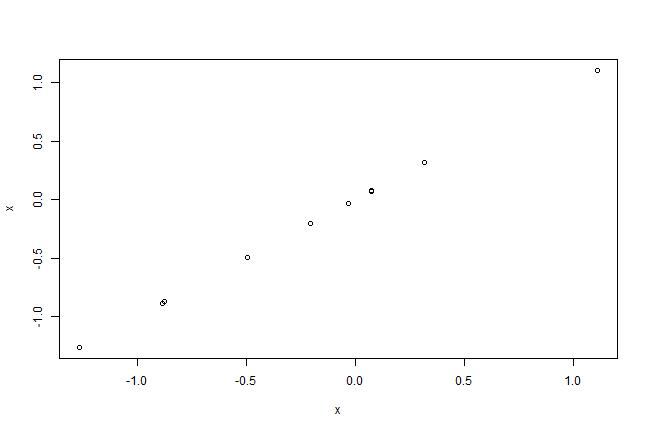
\includegraphics{prezentacja_pakietu_files/figure-beamer/unnamed-chunk-5-1.jpeg}

\end{frame}

\hypertarget{business_card}{%
\section{business\_card()}\label{business_card}}

\begin{frame}[fragile]{business\_Card()}
\protect\hypertarget{business_card-1}{}

business\_card() is converting .Rmd file into beautiful MiNI WUT themed
business card

An example usage:

\scriptsize

\begin{Shaded}
\begin{Highlighting}[]
\NormalTok{rmarkdown}\OperatorTok{::}\KeywordTok{render}\NormalTok{(}
  \StringTok{'tests/business_card/business_card.Rmd'}\NormalTok{, miniBeamer}\OperatorTok{::}\KeywordTok{business_card}\NormalTok{()}
\NormalTok{)}
\end{Highlighting}
\end{Shaded}

\end{frame}

\begin{frame}[fragile]{Example business card}
\protect\hypertarget{example-business-card}{}

\scriptsize

\begin{Shaded}
\begin{Highlighting}[]
\OperatorTok{---}
\NormalTok{address}\OperatorTok{:}\StringTok{ }\ErrorTok{|}
\StringTok{  }\ErrorTok{@}\NormalTok{mckraqs}
\NormalTok{logo}\OperatorTok{:}\StringTok{ "WMiNI-znak.png"}
\NormalTok{person}\OperatorTok{:}
\StringTok{  }\OperatorTok{-}\StringTok{ }\NormalTok{name}\OperatorTok{:}\StringTok{ }\NormalTok{Mateusz Polakowski}
\NormalTok{    title}\OperatorTok{:}\StringTok{ }\NormalTok{Data Science, MiNI PW}
\NormalTok{    phone}\OperatorTok{:}\StringTok{ "+48 997 998 999"}
\NormalTok{    email}\OperatorTok{:}\StringTok{ }\NormalTok{mateusz.polakowski}\OperatorTok{@}\NormalTok{mini.pw.edu.pl}
\NormalTok{    url}\OperatorTok{:}\StringTok{ }\NormalTok{https}\OperatorTok{:}\ErrorTok{//}\NormalTok{github.com}\OperatorTok{/}\NormalTok{mckraqs}\OperatorTok{/}\NormalTok{miniBeamer}
\NormalTok{cols}\OperatorTok{:}\StringTok{ }\DecValTok{1}
\NormalTok{rows}\OperatorTok{:}\StringTok{ }\DecValTok{1}
\NormalTok{output}\OperatorTok{:}\StringTok{ }\NormalTok{miniBeamer}\OperatorTok{::}\NormalTok{business_card}
\OperatorTok{---}
\end{Highlighting}
\end{Shaded}

\end{frame}

\begin{frame}{WOW! WOW! This card is nice!}
\protect\hypertarget{wow-wow-this-card-is-nice}{}

\begin{figure}
\centering

\includegraphics{card.png}
\caption{Business card}
\end{figure}

\end{frame}

% ***
% afterbody.tex template, feel free to use it
% File generated thanks to mckraqs/miniBeamer package!
% ***

\end{document}
